\section{Recognition Problems}

We deal with a dataset of images $\mathcal{D}$, where each image $\mathcal{I}$ contains at least one, and often multiple, objects.
Each object is labeled with exactly one category label $k \in \{1, \dots, K\}$.

The multi-class, multi-label \textbf{classification} problem asks whether $\mathcal{I}$ contains at least one object of class $k$.
The answer for a single label is given with a real-valued confidence by a function $\emph{classify}(\mathcal{I},k)$.
We write the ground truth for an image as $\mathbf{C}=\{C_1,\dots,C_K\}$, where $C_k \in \mathbb{B} = \{0,1\}$ is set to $1$ if an object of class $k$ is present.

The answer is evaluated by plotting precision vs. recall across dataset $\mathcal{D}$ (by progressively lowering the confidence threshold for a positive label) and integrating to yield the Average Precision (AP) metric, which has become the standard evaluation for recognition performance on challenging datasets \cite{pascal-voc-2010}.

\comment{
We can make the classification problem more difficult by posing the \emph{counting} problem, which asks how many objects of class $k$ are present in $\mathcal{I}$, for each $k$.
This setting is not commonly evaluated; we mention it for its usefulness in later exposition.
}

The \textbf{detection} problem is to output a list of bounding boxes (sub-images defined by four coordinates), each with a real-valued confidence that it encloses a single instance of an object of class $k$, for each $k$.
The answer for a single class is given by an algorithm $\emph{detect}(\mathcal{I},k)$, which outputs a list of sub-image bounding boxes $B$ and their associated confidences.

A common measure of a correct detection is the PASCAL overlap: two bounding boxes are considered to match if they have the same label and the ratio of their intersection to their union is at least $\frac{1}{2}$.
Again, Average Precision is the single-number metric for the performance of a detector.

As our task is fundamentally in \emph{multi-class} object detection, we rely on a slightly different evaluation than is commonly used (although it has precedent in \cite{Desai2009}).
Instead of pooling detections across images in the dataset, and considering classes individually, we pool detections across classes, but consider images individually, reporting results averaged across the dataset.

To highlight the hierarchical structure of these problems, we note that (1) the confidences for each sub-image $b \in B$ may be given by $\emph{classify}(b,k)$; (2) the correct answer to the detection problem also answers the classification problem. \comment{the counting and classification problems}

Our goal is a general recognition policy that outputs both classification and detection results; we evaluate on both tasks.

\section{Multi-class Recognition Policy} \label{sec:tech}
\begin{figure}[h!]
\center{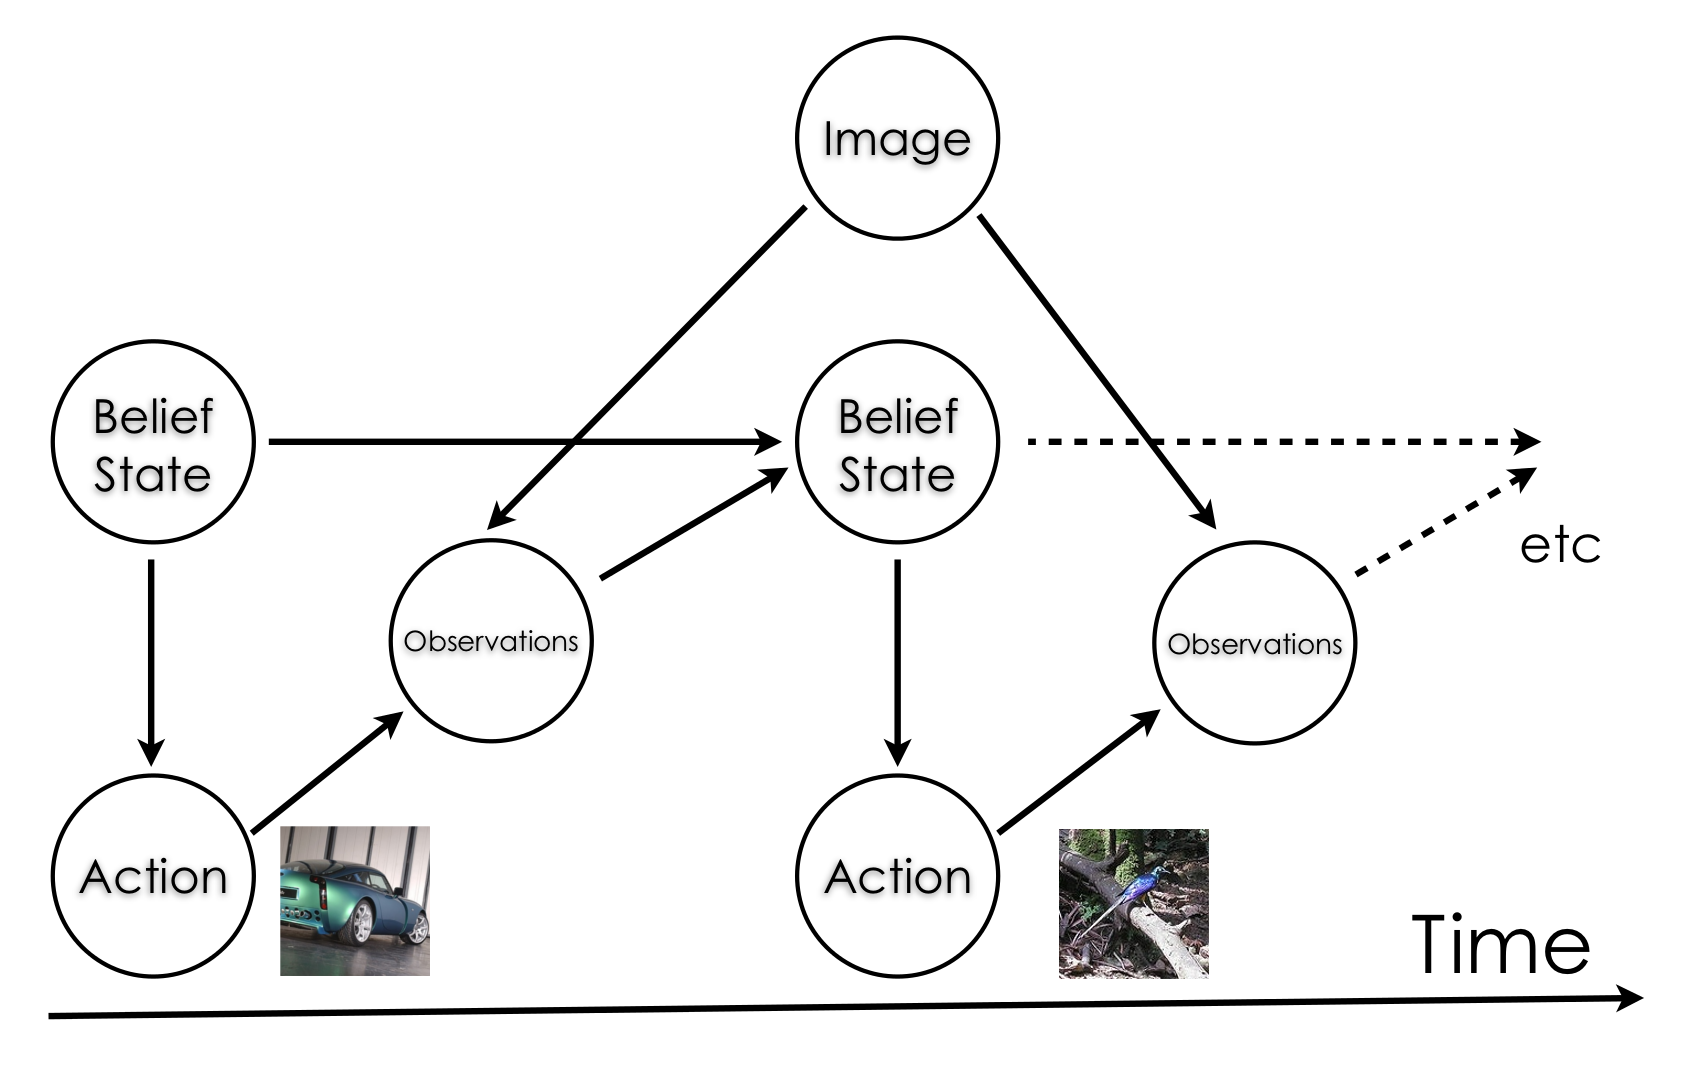
\includegraphics[width=0.66\linewidth]
    {figures/pomdp.png}}
  \caption{Summary of our approach to the problem. Our system has two major parts: (1) selecting an action by predicting its value; (2) updating the belief state with observations resulting from the action.}
  \label{fig:pomdp}
\end{figure}

As presented in Figure~\ref{fig:pomdp}, our goal is a multi-class recognition policy $\pi$ that takes an image $\mathcal{I}$ and then outputs $\{\emph{classify}(1), \dots, \emph{classify}(K)\}$ and a list of multi-class detection results $\emph{detect}(I)$.

The policy repeatedly selects an action $a_i$ from a set of actions $\mathcal{A}$, executes it, potentially receives an observation $o_i$, and selects the next action.
The set of actions can include classifiers, detectors, or hybrid actions (detector followed by classification of its output).

A dynamic, or ``closed-loop,'' policy bases action selection on observations received from previous actions, exploiting the signal in inter-object and scene context for a maximally efficient path through the actions.
This is our goal, and what sets our formulation apart from multi-class systems that evaluate in a fixed order, such as simple cascades \cite{Viola2001} or decision trees.

Let $\mathcal{A}$ consist of $K$ detectors $L^\text{det}_i$.
We use one-vs-all deformable part-model classifiers on a HOG featurization of the image \cite{Felzenszwalb2010a}, with associated linear classification of the detections.

\comment{Let $\mathcal{A}$ consist of $K$ actions:
\begin{itemize}
  \item $K$ detectors $L^\text{det}_i$: one-vs-all deformable part-model classifiers on a HOG featurization of the image \cite{Felzenszwalb2010a}, with associated linear classification of the detections.
  \item $K$ classifiers $L^\text{gist}_i$: one-vs-all SVMs on the GIST feature \cite{Torralba2004}.
\end{itemize}}

\subsubsection{Time and Evaluation}
Each action $L$ has an expected cost $c(\cdot)$ of execution.
Depending on the setting, the cost can be defined in terms of algorithmic runtime analysis, an idealized property such as number of \emph{flops}, or simply the empirical runtime on specific hardware.
We take the empirical approach: every executed action advances $t$, the \emph{time into episode}, by its empirical runtime.

As shown in Figure~\ref{fig:evaluation}, the system is given two times: the setup time $T_s$ and deadline $T_d$.
From the setup time to the deadline, we want to obtain the best possible answer if stopped at any given time.
This corresponds to the general notion of \emph{Anytime} algorithms, and is motivated by desired flexibility in the system.

A single-number metric that corresponds to this objective is simply the ratio of the area captured under the curve to the total area between the start and deadline bounds.
\comment{Just like the metric of Average Precision itself was motivated by the inadequacy of any single Precision-Recall operating point to describe the performance of a robust system, our proposed metric is motivated by the inadequacy of any single Performance vs. Time operating point.}
We evaluate policies by this more robust metric and not simply by the final performance at deadline time for the same reason that Average Precision is used instead of a fixed Precision vs. Recall point.

\subsubsection{Sequential Execution}
An action $a_i$ that consists of running a classifier $L_i$ returns a real-valued observation $o_i \sim P(O_i)$.
The state records the fact that $a$ has been taken by adding it to the initially empty set $\mathcal{O}$.
We refer to the current set of observations as $\mathbf{o} = \{o_i | L_i \in \mathcal{O}\}$.

We define the belief state $b$ of the decision process by the the distribution over class presence variables $P(\mathbf{C}) = P(C_1, \dots, C_K)$, where we write $P(C_k)$ to mean $P(C_k=1)$.
Additionally, $b$ records the time into episode $t$, and the set of executed actions $\mathcal{O}$ with corresponding observations $\mathbf{o}$.

A recognition \emph{episode} takes an image $\mathcal{I}$ and proceeds from the initial belief state $b^0$ and action $a^0$ to the next pair $b^1$, and so on until $t$ exceeds $T_d$.
At that point, the policy is terminated and a new episode begins on a new image.

The policy's performance at time $t$ is determined by the detection and classification observations that have been observed at the last belief state $b^j$ before that point.
For classification of unobserved classes, we treat the corresponding values of $P(\mathbf{C})$ as the set of confidence scores $\{\emph{classify}(k)\}$.
Detection results of unobserved classes are an empty set.

Our notation is summarized in \autoref{tab:notation}.

\begin{table}[h!]
\centering
\caption{Summary of the notation.}
\label{tab:notation}
\begin{tabular}{|l|l|}
  \hline
  $\mathcal{I}$ & image \\
  $C_k$         & presence of class $k \in \{1,\dots,K\}$ \\ 
  $t$           & time into episode \\ 
  $T_s$, $T_d$  & start and deadline times \\ 
  $b^j$         & belief state at step $j$ \\ 
  $\pi$         & policy function, $b \mapsto a \in \mathcal{A}$ \\
  $\mathcal{A}$ & set of actions $a$\\ 
  \comment{$\mathcal{F}$ & set of featurization actions \\}
  \comment{$\mathcal{L}$ & set of classification actions\\}
  $o_i$         & a real-valued observation upon executing $a_i \in \mathcal{A}$\\
  $\mathcal{O}$ & set of executed actions\\
  $\mathbf{o}$  & set of observations $\{o_i | a_i \in \mathcal{O}\}$\\
  $c(a_i)$        & cost of executing $a_i$, in units of $t$\\
  \hline
\end{tabular}\end{table}

\section{Selecting actions} \label{sec:value}
\comment{Optimal performance results from becoming maximally certain of the correct values $C_i$ as quickly as possible (given the setup time).}
As our goal is to pick actions dynamically, we want to formulate a function $V(b,a)$  that assigns a value to a potential action, given the current state of the decision process.
We can then define the policy as simply the untaken action with the maximum value:
\begin{align}
\pi(b) = \argmax_{a_i \in \mathcal{A} \setminus \mathcal{O}} V(b,a_i)
\end{align}

For this policy to be \emph{closed-loop}, the observations $o_i$ generated by taking an action $a_i$ need to update $b$ and thus influence the selection of the next action.
Figure~\ref{fig:pomdp} visualizes such an execution process.

One simple heuristic value function that we can try is simply picking the action corresponding to the class presence variable $C_k$ with the highest probability.
Of course, we'd like to learn the value function from the data, but the above heuristic will be used as a baseline in the evaluation to follow.

Before we discuss how to set $V(b,a_i)$ such that our policy obtains best performance under our evaluation, we present our model for updating the belief state with observations.

\subsection{The model of the belief state}
\begin{figure}[h!]
\centering
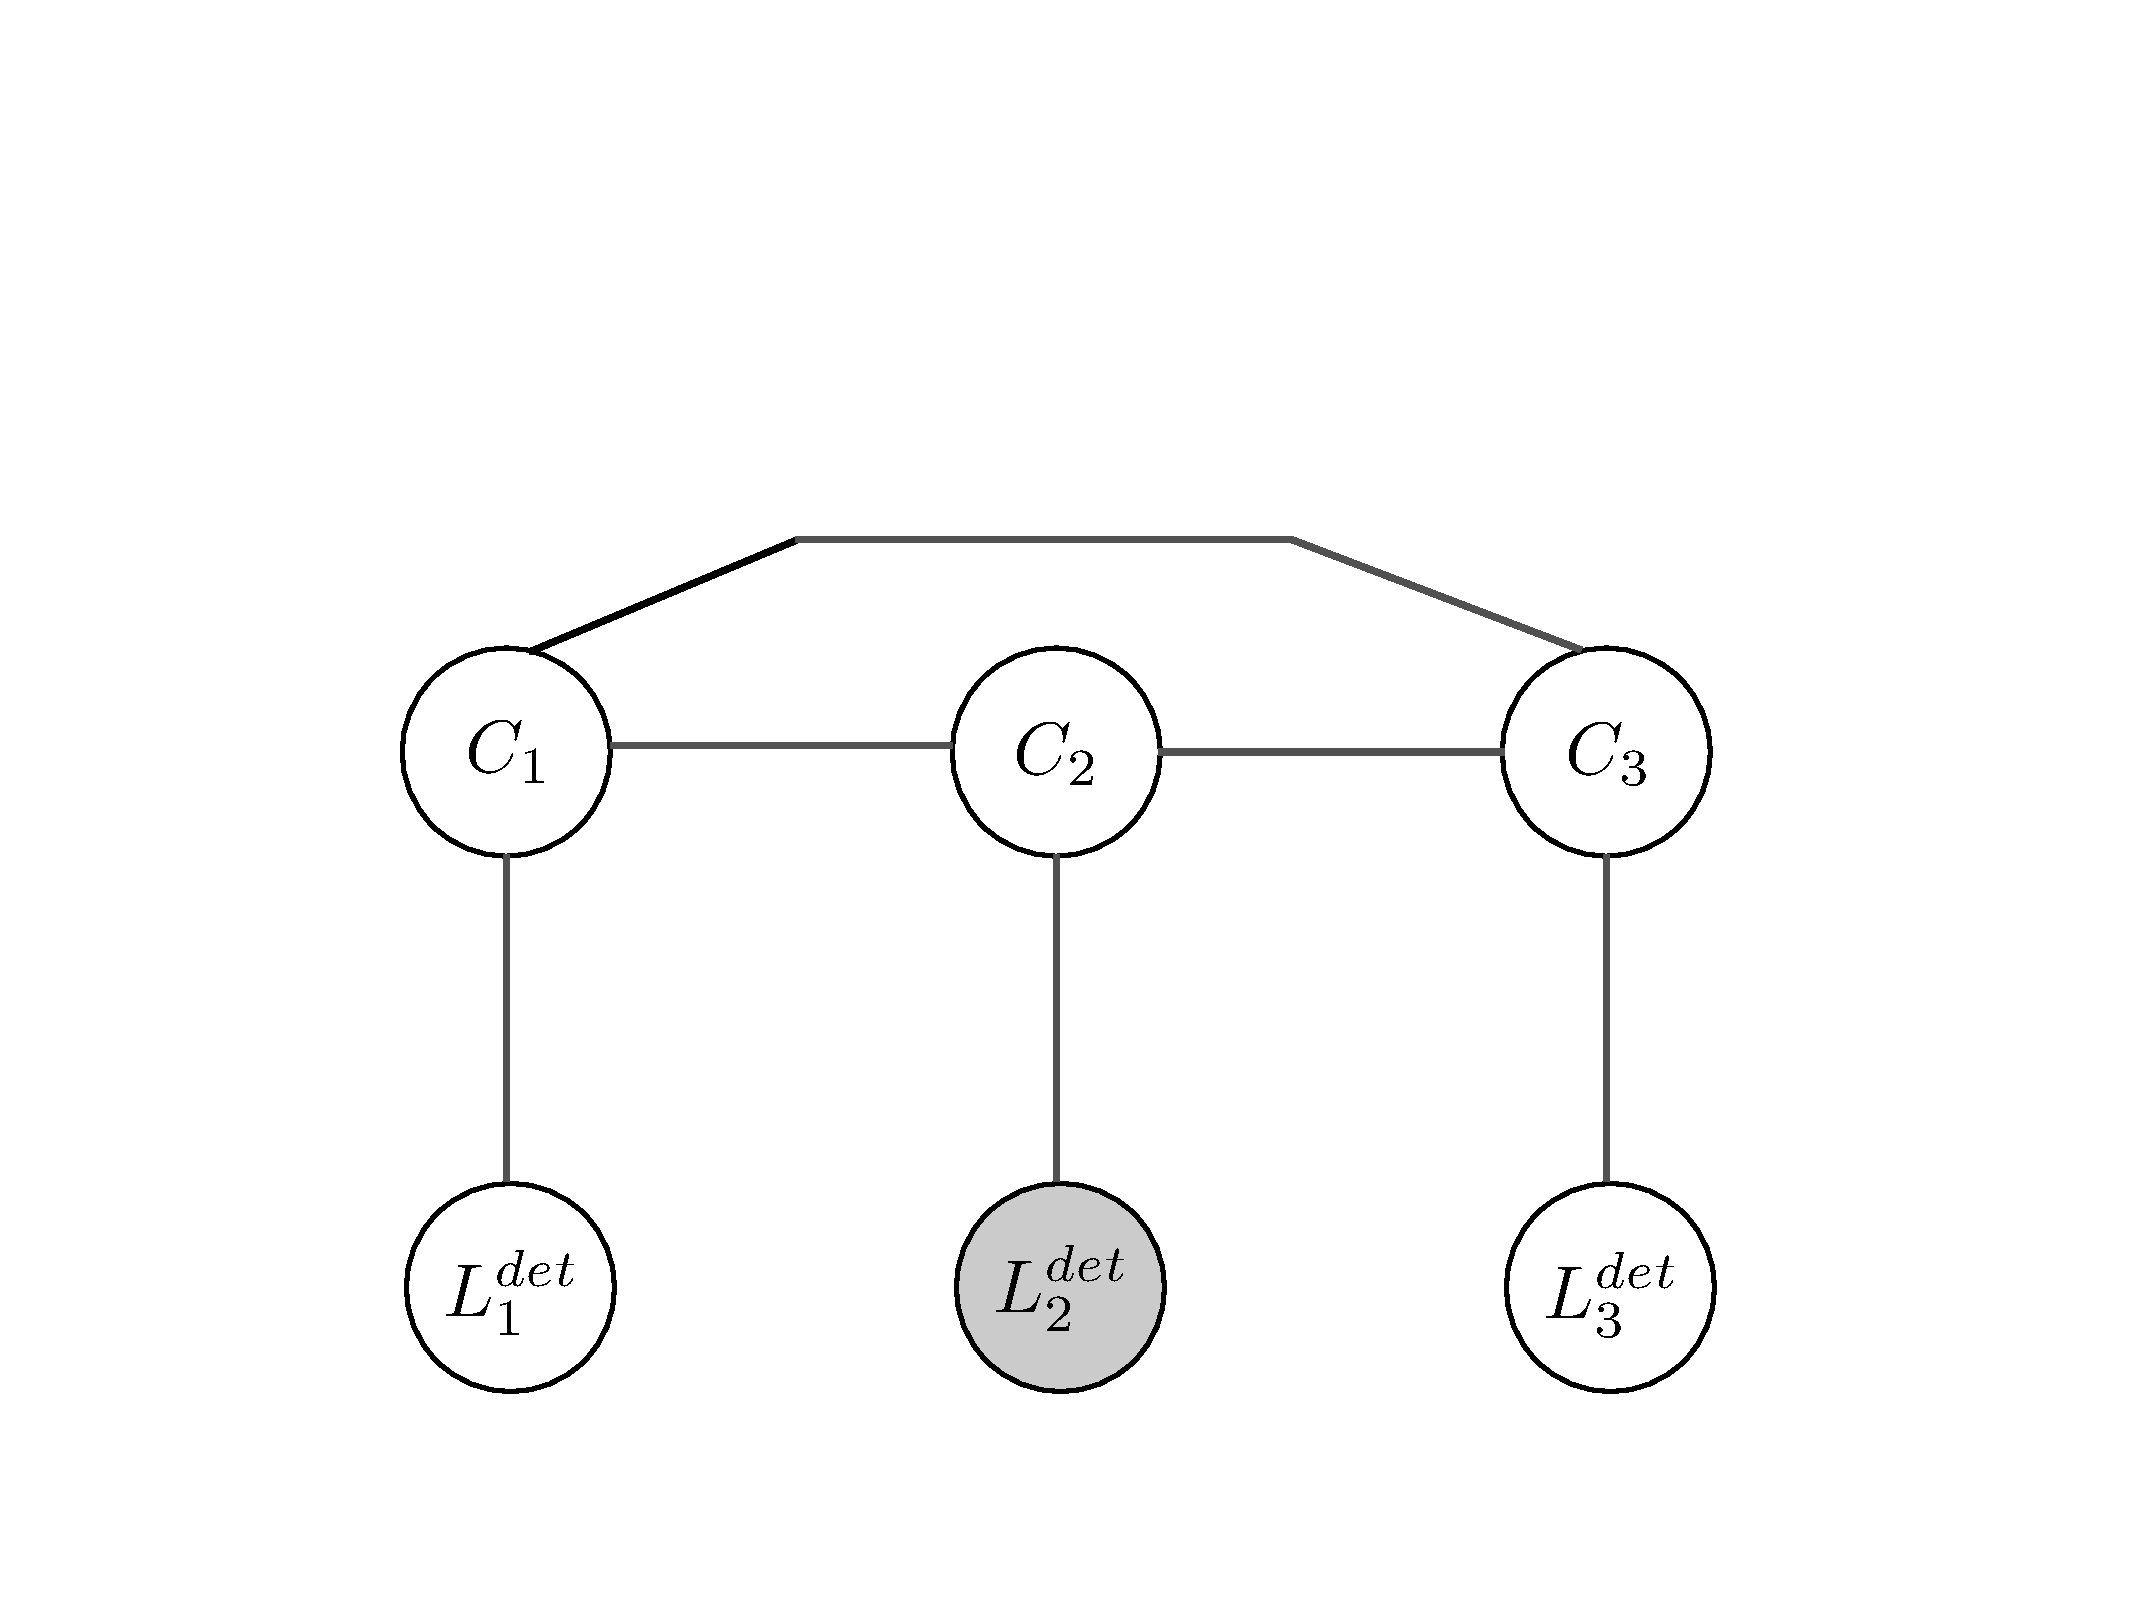
\includegraphics[width=0.56\linewidth]{figures/inf_model_mrf_1.pdf}
\caption{
The MRF inference model used in our system.
We show a point in the middle of the decision process for 3 classes; one action has already been taken.
\comment{Some classifiers have already been observed.}
}
\label{fig:model}
\end{figure}

The quantities that may be useful to us for selecting which actions to deploy are the probabilities and entropies of the class presence variables $C_k$.
These allow us to look for the most probable classes given the observations.
When the policy starts, the model should present the prior distributions $P(C_k)$; as observations are accrued, the model should present the updated conditionals $P(C_k|\mathbf{o})$.

We employ a fully-connected Markov Random Field (MRF), as shown in Figure~\ref{fig:model}.
The $L_i$ variables are discretized from real-valued responses of a classifier on the detections output by the deformable part-model detector we employ (see Section~\ref{sec:tech}).

The classifier is a linear kernel SVM on the top two max detection scores in the list of detections.
The responses are discretized per variable based on the distribution of the scores on the training dataset.

The MRF is implemented with an open-source graphical model package \cite{Jaimovich2010}.
The parameters of the model are trained on fully-observed data.
Exact inference is generally intractable in this model.
Instead, we use Loopy Belief Propagation, which does not provide general convergence guarantees but has been shown to work well empirically on similar tasks \cite{Desai2009}.

\subsection{Learning the Value Function}

Remember that our heuristic value function consisted of picking the action corresponding to the class presence variable with the highest probability $P(C_k)$.
We can formulate such a policy as a scalar product:
\begin{align}
\pi(b) = \argmax_{a_i \in \mathcal{A} \setminus \mathcal{O}} \theta^\top \phi(b,a_i)
\end{align}
where $\phi(b,a_i)$ is a feature vector representation of the belief state.
This approach is known as function approximation in reinforcement learning \cite{Sutton1998}.

Let us take take the feature representation for an action $a_i$ to be $[P(C_k), \, 1]$, where $C_k$ corresponds to the action.
This corresponds to our heuristic value function, with a bias variable.
The feature representation $\phi(b,a_i)$ then is a vector of size $F|\mathcal{A}|$, with $F=2$ for this feature, where all values are $0$ except those corresponding to $a_i$.

This representation allows us to use a single vector of weights $\theta$ as a compact representation of our policy.

At each time step, our system is evaluated by properties of the state $b$ (the list of detections and the classification outputs).
The final evaluation metric is a function of the history of execution $h^0=b^0,b^1,\dots,b^J$, with $J$ being the last step of the process with $t \le T_d$.

Ideally, the value function for a point in the decision process $b^j$ should give the expected value of the final evaluation metric, over all possible histories starting at point $j$:
\begin{align}
V(b^j,a_i) = \mathbb{E}_{h^j \sim P(h^j|b,a_i)}[R(h^j)]
\end{align}

The reward function $R(h^j)$ assigns a real-valued score to a history.
We have considerable flexibility in defining $R$; it does not necessarily have to be directly tied to the final evaluation.

One feature we want the reward function to have is additivity.
Let's say that given deadline $T_d$ and some image, the policy had time to take $J$ actions.
The total reward of a policy $\pi$ starting at state $b^j$ is then defined as the sum of rewards
\begin{equation}
R(h^j) = \sum_{j'=j}^J R(b_j',a^{j'})
\end{equation}

We formulate two reward definitions: one strives to match the final AP evaluation of the detections, and one is motivated by lowering uncertainty of $P(\mathbf{C})$.

\subsubsection{Reward: area under the AP vs. Time curve}
\begin{figure}[htb]
  \centering
  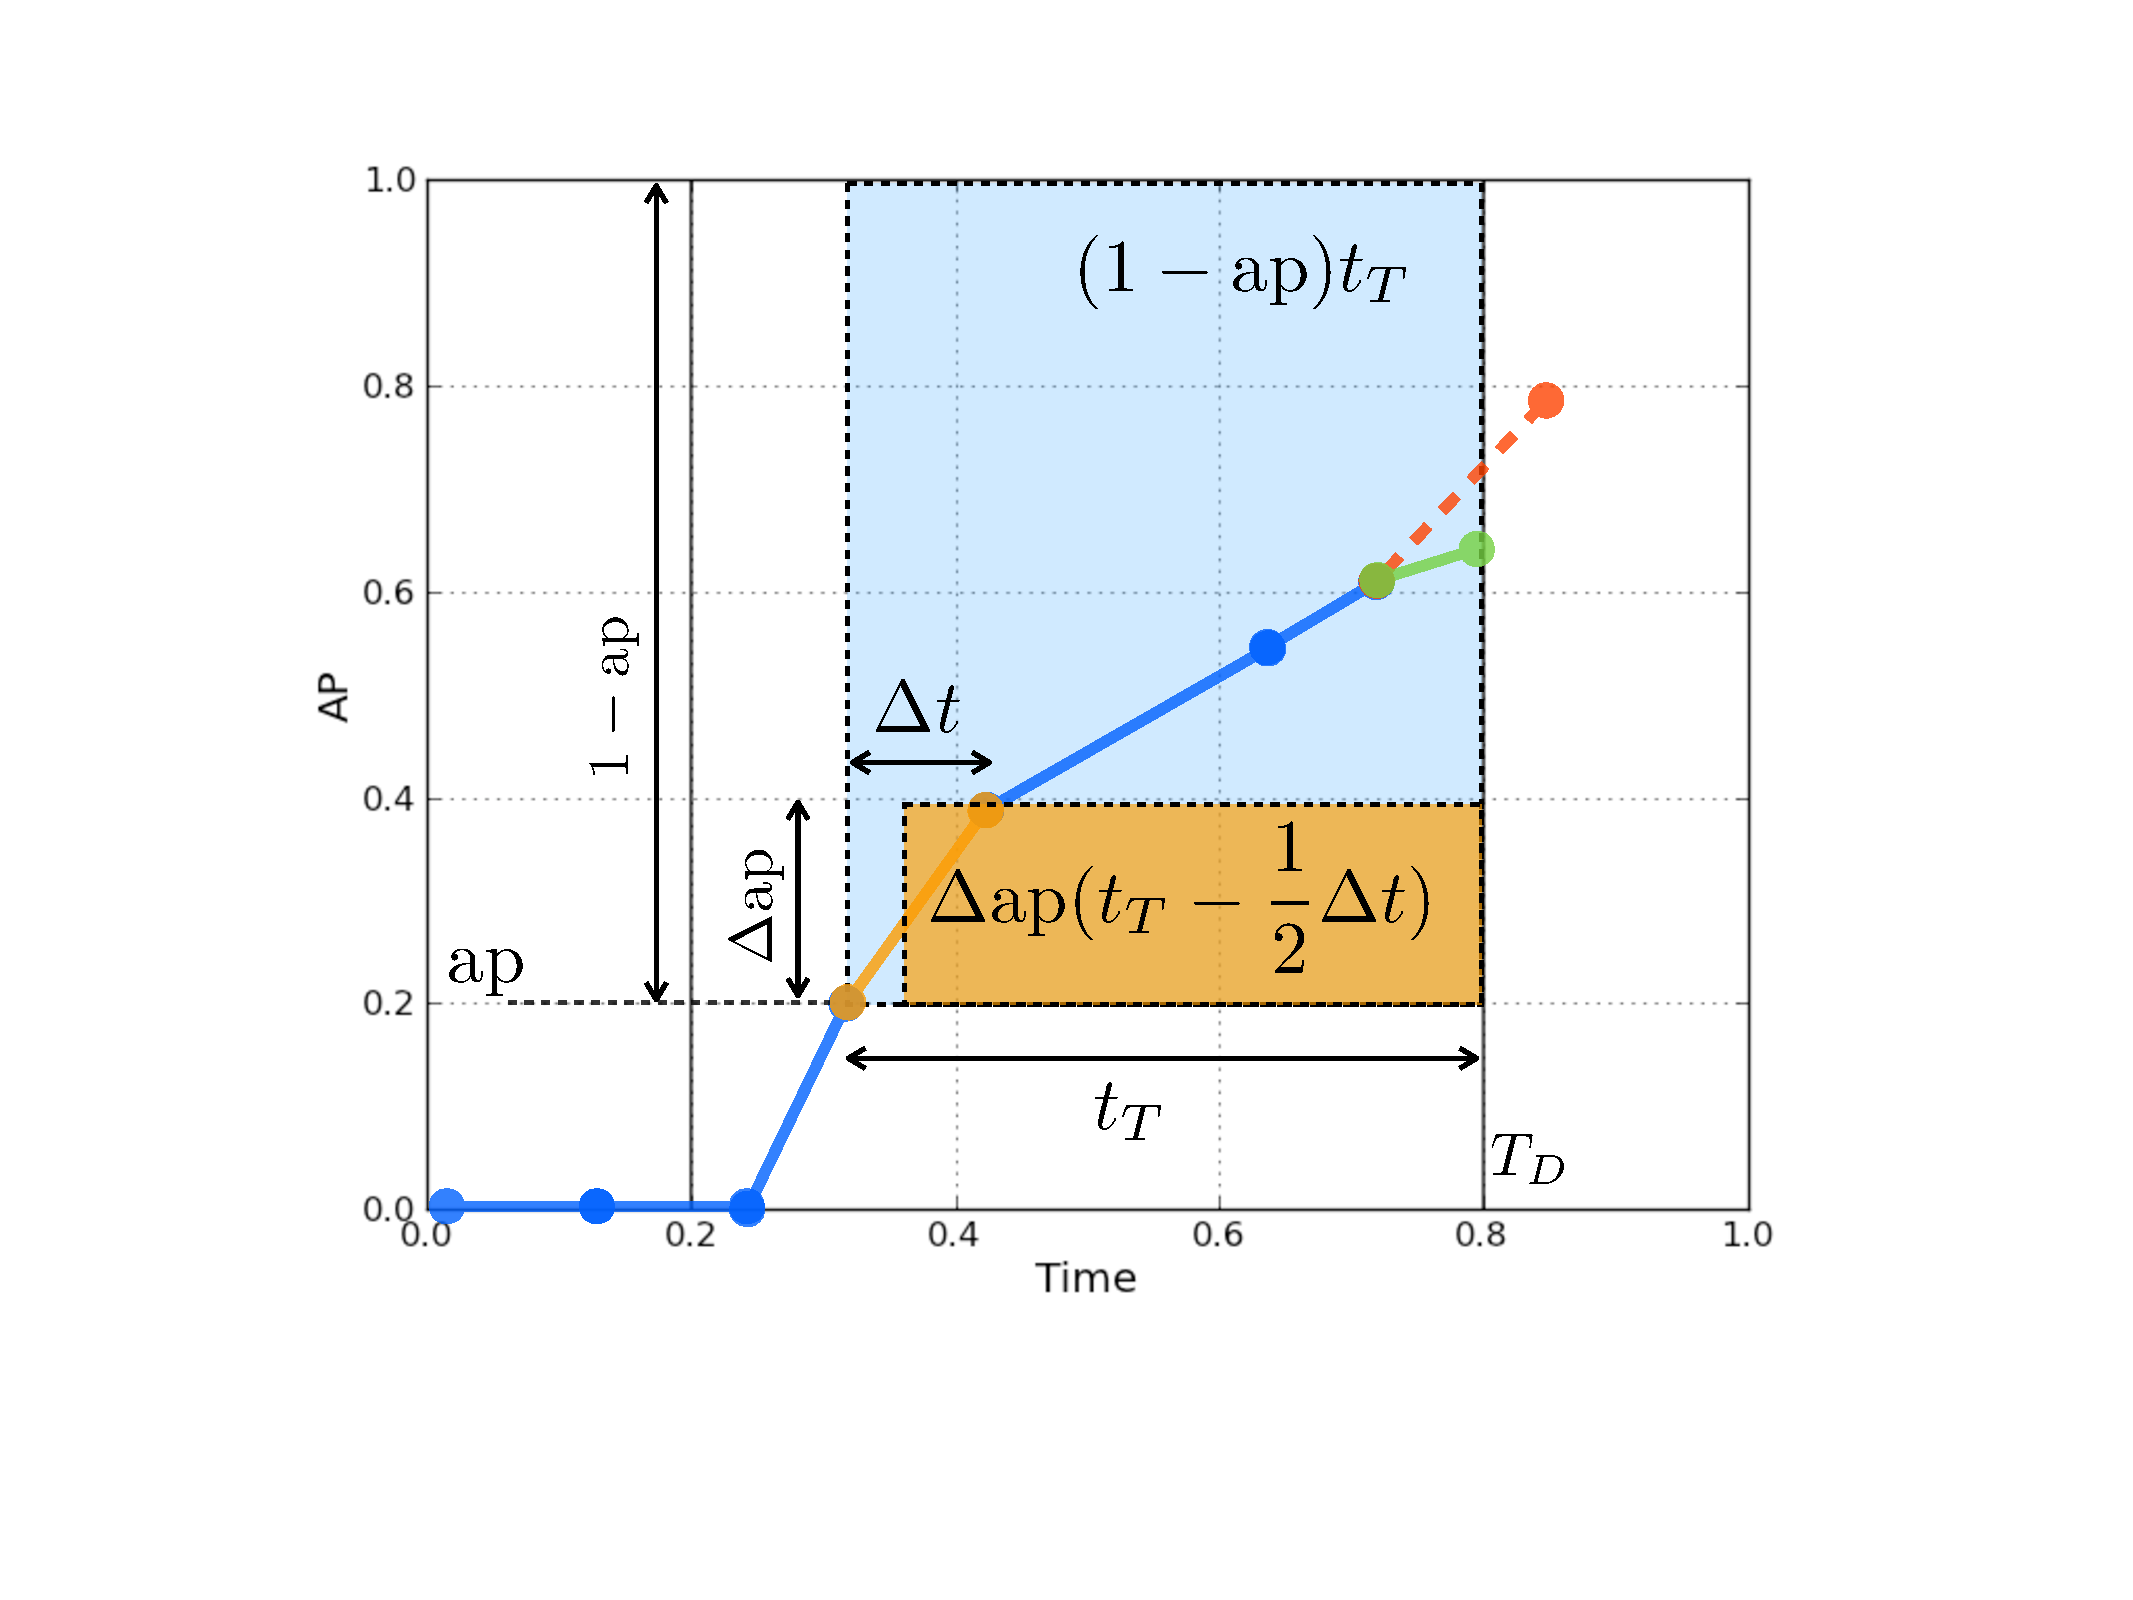
\includegraphics[width=0.56\linewidth]{figures/apvst_expl.pdf}
  \caption{A per-action greedy value function that corresponds to the maximization of our objective function is the area of the horizontal slice under the curve due to the action. The figure shows this analysis for the action highlighted in orange.}
  \label{fig:rewards}
\end{figure}

The final evaluation of a policy consists of the area under the performance vs. time curve (normalized by the total area).
Accordingly, we formulate per-action rewards such that their addition results in this quantity.

Specifically, as shown in Figure~\ref{fig:rewards}, we define the reward of an action as
\begin{equation}\label{eq:advanced}
R(b^j,a_i) = \frac{\Delta \text{ap}_i (t_T^j-\frac{1}{2}\Delta t_i)}{(1-\text{ap}^j)t_T^j}
\end{equation}
where $t_T^j$ and $\text{ap}^j$ are the time left until deadline and the AP at state $b^j$, and $\Delta t_i$ and $\Delta \text{ap}_i$ are the time taken and AP change produced by the action $a_i$.

The reward is $1$ if the policy takes an action that obtains the maximum possible area under the curve at that point, and $0$ if no area under the curve is captured.

\subsubsection{Reward: decrease in mean entropy}
We also consider a similar additive reward function based on the mean entropy of the variables $P(C_k)$: $\frac{1}{K}\sum_{k=1}^K H(C_k)$, where $H(C_k) = - \sum_{c_k \in {0,1}} P(c_k) \log P(c_k)$.
We follow the same setup as above, but strive to maximize the area \emph{above} the curve of mean entropy vs. time.

The goal of a policy that maximizes these rewards is to take actions that reduce uncertainty of the most uncertain variables most quickly.

\subsection{Learning the weights}

The feature representation of the belief state for a given action $a_i$ that corresponds to class $k$ is defined to be
\begin{align}
\phi_k(b) = [P(C_k), \, H(C_k), \, 1]
\end{align}

Our procedure for learning the weights is standard generalized policy iteration \cite{Sutton1998}.
We first initialize the weights $\theta$ to the heuristic value function of simply picking the maximum $P(C_k)$: $\theta_i = [1, \,0, \,0]$.

With this policy, we run $N$ recognition episodes.
From the state-action samples gathered in running the episodes, we formulate a matrix $\Phi$ from the featurizations $\phi(b^j,a_i)$, and a vector $y$ consisting of the individual rewards $R(b^j,a_i)$.

The rewards are computed as the sum of discounted rewards to the end of the episode:
\begin{align}
R(b^j,a_i) = \sum_{i=0}^{J-j} \lambda^i R(b_{j+i},a^{j+i})
\end{align}
Note that with $\lambda=0$, the reward is determined entirely by the actual action taken; with $\lambda=1$, the reward is the sum of all rewards until the end of the episode.

We then solve the system $\Phi \theta = y$ for $\theta$ with Lasso regression.
With the updated weights $\theta$, we run $N$ more episodes and repeat the procedure until convergence.

The parameters of this training procedure are the $\alpha$ weight on the regularization term in the regression and the $\lambda$ discount weight.
We cross-validate for both values.
